\chapter{羔羊展開書卷（6:1-7:17）}
羔羊在天上揭印，地上展開審判。
前四印給地上的審判是戰爭、饑荒與死亡。第五印轉向為上帝的道和作見證而殉道的聖徒。第六印揭開之後，天地震動、星辰墜落。羔羊忿怒的大日來到。地上的人驚問：「誰能站得住？」所以啟示錄第七章回答這個問題：唯有蒙羔羊寶血潔淨、屬於神的百姓，才能站在寶座和羔羊面前。因此，七印不僅揭示可畏的審判，也見證神對祂子民的保守，以及羔羊所成就的救恩與永恆盼望。

\section{第一印到第四印：四騎士}

\begin{ScriptureBox2}{圈出每匹馬的顏色，並劃出每位騎馬者被賜予的或所做的事。每匹馬出來以前，是誰揭開每一印？}

\item[6:1] 我看見羔羊揭開七印中第一印的時候、就聽見四活物中的一個活物、聲音如雷、說、你來。

\item[6:2] 我就觀看、見有一匹白馬、騎在馬上的拿著弓．並有冠冕賜給他．他便出來、勝了又要勝。

\item[6:3] 揭開第二印的時候、我聽見第二個活物說、你來。

\item[6:4] 就另有一匹馬出來、是紅的．有權柄給了那騎馬的、可以從地上奪去太平、使人彼此相殺．又有一把大刀賜給他。

\item[6:5] 揭開第三印的時候、我聽見第三個活物說、你來。我就觀看、見有一匹黑馬．騎在馬上的手裡拿著天平。

\item[6:6] 我聽見在四活物中、似乎有聲音說、一錢銀子買一升麥子、一錢銀子買三升大麥．油和酒不可蹧蹋。

\item[6:7] 揭開第四印的時候、我聽見第四個活物說、你來。

\item[6:8] 我就觀看、見有一匹灰色馬．騎在馬上的、名字叫作死．陰府也隨著他．有權柄賜給他們、可以用刀劍、饑荒、瘟疫、〔瘟疫或作死亡〕野獸、殺害地上四分之一的人。
\end{ScriptureBox2}

\begin{figure}[htbp]
    \centering
    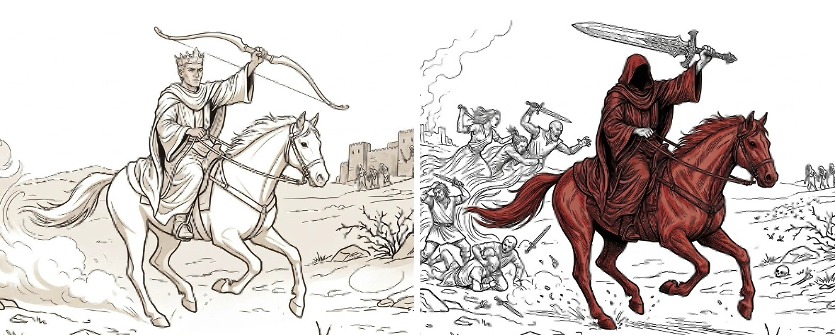
\includegraphics[
    width=1\textwidth, 
    trim=0 0 0 00, 
    clip]{images/horses_white_red.png}
    \caption{第一、二印：白馬勝、紅馬殺}
    \label{fig:horses_white_red.png}
\end{figure}

四匹馬和騎士，帶來地上接連出現的征服、戰爭、饑荒與死亡。
白馬是勝了又勝，紅馬帶來殺戮。
黑馬帶來飢荒使人貧窮，灰馬帶來死亡。
我使用一個口訣，記住它們的特徵。
\begin{center}
\begin{tabular}{ll}
\hline
中文 & English \\
\hline
白馬勝 & White to conquer \\
紅馬殺 & Red to kill \\
黑馬窮 & Black to famine \\
灰馬死 & Pale to die
\end{tabular}
\end{center}


\begin{figure}[htbp]
    \centering
    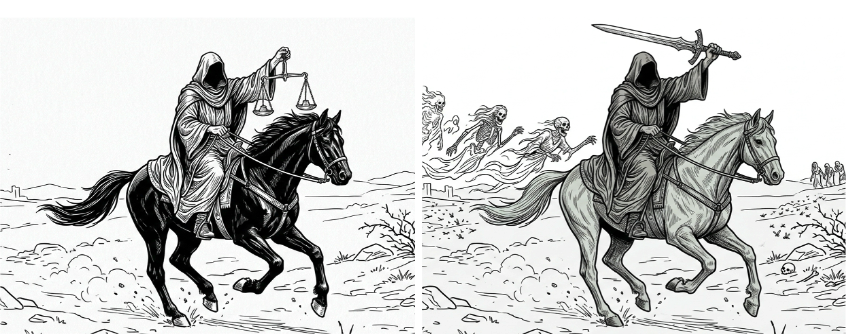
\includegraphics[
    width=1\textwidth, 
    trim=0 0 0 0, 
    clip]{images/horses_black_gray.png}
    \caption{第三、四印：黑馬窮、灰馬死}
    \label{fig:horses_black_gray.png}
\end{figure}

「一錢銀子買一升麥子」形容戰爭之後隨之而來的饑荒，糧食匱乏，物價暴漲。戰爭期間，軍隊往往透過掠奪鄉村取得糧食，甚至以武力奪取食物，使鄉野遭到洗劫。饑荒便成為戰爭帶來的嚴重後果之一。

小麥和大麥是羅馬帝國重要的糧食來源。小麥品質較好，是主要的主食；大麥價格較低，通常是較貧困者食用的穀物。一升小麥大約足夠一個人一天的口糧，而三升大麥則大致相當於一個人一天的口糧。

「一錢銀子」（denarius）通常相當於一個工人一天的工資。因此，一個人辛苦工作一整天，所得幾乎只夠購買自己一天所需的小麥；若買大麥，也只能勉強維持基本的口糧。若還要養活家人，支付住房及其他日常開銷，便更加困難。這正是經文所描繪的饑荒景況：糧食仍然可以買到，卻已昂貴到一般人難以負擔。
至於更稀缺的橄欖油和酒，在糧食匱乏的時候，更是「不可蹧蹋。」

紅、黑、灰馬在經文中寫的相當清楚，那白馬是誰呢？解經家一般有三種解釋。
{
\small
\renewcommand{\arraystretch}{1.1}
\setlength{\tabcolsep}{4pt}
\begin{longtable}{>{\raggedright\arraybackslash}p{2.4cm}|
                  >{\raggedright\arraybackslash}p{7.2cm}}
\caption{白馬騎士的三種解釋}
\label{tab:white-horse} \\
\hline
解釋 & 主要理由 \\
\hline
\endfirsthead

\multicolumn{2}{l}{\small\itshape 表~\thetable（續）} \\
\hline
解釋 & 主要理由 \\
\hline
\endhead

\hline
\endfoot

\hline
\endlastfoot

代表假基督或敵基督勢力

\smallskip
{\color{burgundy}\small\faStar} &
這是許多未來論（Futurist）解經家所持的觀點，見「附錄：各種末世論觀點」。\footnote{MacArthur, J. (2007).}
因為白馬騎士拿著弓，卻沒有提到箭，象徵用欺騙或政治手段征服，並且啟示錄後面出現獸和敵基督的勢力。因此有些解經者認為第一印是末世敵基督活動的開始。馬太福音 24:4-5 先提到假基督迷惑多人，之後才提到戰爭和饑荒，次序與四騎士相近。 \\
\hline
代表軍事征服 &
有些解經者認為白馬不一定是敵基督，因為經文直接提到「勝了又要勝」，所以他們認為是象徵一般性的軍事擴張與帝國征服。征服往往引發戰爭、饑荒和死亡。後面的紅馬、黑馬和灰馬都是有關於戰爭、饑荒和死亡的災難。 \\
\hline
代表基督或福音得勝 &
這是較少數的觀點。支持者認為白色在啟示錄中常象徵聖潔與得勝，因爲啟示錄 19:11 的基督也是騎著白馬。「勝了又要勝」可理解為福音不斷擴展。
可是多數現代解經者不同意此觀點，因為四騎士是一組，應當一起看。而且此處的白馬騎士與啟示錄19章白馬上的基督之間仍存在許多差異。 \\
\end{longtable}
}
\section{第五印：殉道者的呼求}

\begin{ScriptureBox2}{劃出這些人被殺的原因。他們向主求什麼？他們得著什麼，又被告知什麼？}
\item[6:9] 揭開第五印的時候、我看見在祭壇底下、有為　神的道、並為作見證、被殺之人的靈魂．

\item[6:10] 大聲喊著說、聖潔真實的主阿、你不審判住在地上的人給我們伸流血的冤、要等到幾時呢。

\item[6:11] 於是有白衣賜給他們各人．又有話對他們說、還要安息片時、等著一同作僕人的、和他們的弟兄、也像他們被殺、滿足了數目。
\end{ScriptureBox2}

在羅馬人眼中，耶穌的跟隨者是迷信的，為了效忠一位被釘十字架的彌賽亞而犧牲性命，是荒謬可笑的。歷史上的記載也是如此。\footnote{Koester, C. R. (2014).}\footnote{Tacitus, \textit{Ann.} 15.44（塔西佗，《編年史》15.44）；Pliny the Younger, \textit{Ep.} 10.96.8（小普林尼，《書信集》10.96.8）。}\footnote{\textit{Mart. Carp.} 9（《卡爾波殉道記》9）。}

殉道者是「為神的道」並且「作見證」就被殺害。也就是說，他們是專心教導神純全的話語，並做個人見證，這樣子就被殺害，可見是多麼的不公不義。

這段經文對於第一世紀殉道的基督徒，是何等的安慰。祭壇底下的殉道者雖然在地上遭人拒絕，卻蒙上帝悅納。
殉道者的呼求，使我們學到：

\begin{ReaderQuestion}[殉道者給我們的三個功課]
\begin{enumerate}
\item 忠心作見證，即使付上生命的代價（6:9）。
\item 將冤屈帶到聖潔、公義的主面前（6:10）。
\item 在尚未完全成就的公義中，領受上帝的肯定，繼續忍耐等候（6:11）。
\end{enumerate}

\smallskip
這三個功課中，哪一個是你現在最難活出來的？這週你可以怎樣實踐它？
\end{ReaderQuestion}

可是，你可能會問主耶穌不是教導我們要愛仇敵，為逼迫我們的人禱告嗎？那麼，我們該如何理解殉道者的呼求呢？這裡的關鍵在於，我們是否也看見了受害者所承受的不義。

這些殉道者因忠於基督而遭受逼迫，甚至被殺害。他們求上帝伸冤，並不是要親自報復，而是將審判交託給公義的上帝。這段經文說的是一位公義的上帝，也不會忘記那些忠心跟隨祂、為祂作見證的人。
如果殉道者所承認的上帝是「聖潔真實」的，那麼，當惡人殺害無辜者、流無辜人的血時，上帝難道會一直袖手旁觀嗎？
\footnote{Koester, C. R. (2014)}

神的審判有祂所定的時候，甚至要等到殉道者的數目滿足了，才進入祂所定的終局。

神沒有立即執行最後的審判，並不表示祂忽略罪惡或耽延應許，而是因著祂的憐憫與寬容，仍然給人悔改的機會。正如彼得後書 3:9–10 所說：
「主所應許的尚未成就、有人以為他是耽延．其實不是耽延、乃是寬容你們、不願有一人沉淪、乃願人人都悔改。
但主的日子要像賊來到一樣．那日天必大有響聲廢去、有形質的都要被烈火銷化、地和其上的物都要燒盡了。」

\begin{ReaderQuestion}
當我們面對不公義時，可以如何效法第五印的殉道者呢？
\end{ReaderQuestion}

\section{第六印：星辰落地}

\begin{ScriptureBox2}{圈出每一個被震動的受造之物，並劃出每一群躲藏的人。他們在躲避誰的面目？}
\item[6:12] 揭開第六印的時候、我又看見地大震動．日頭變黑像毛布、滿月變紅像血．

\item[6:13] 天上的星辰墜落於地、如同無花果樹被大風搖動、落下未熟的果子一樣。

\item[6:14] 天就挪移、好像書卷被捲起來．山嶺海島都被挪移離開本位。

\item[6:15] 地上的君王、臣宰、將軍、富戶、壯士、和一切為奴的、自主的、都藏在山洞、和巖石穴裡．

\item[6:16] 向山和巖石說、倒在我們身上罷、把我們藏起來、躲避坐寶座者的面目、和羔羊的忿怒．

\item[6:17] 因為他們忿怒的大日到了、誰能站得住呢。
\end{ScriptureBox2}

\begin{figure}[htbp]
    \centering
    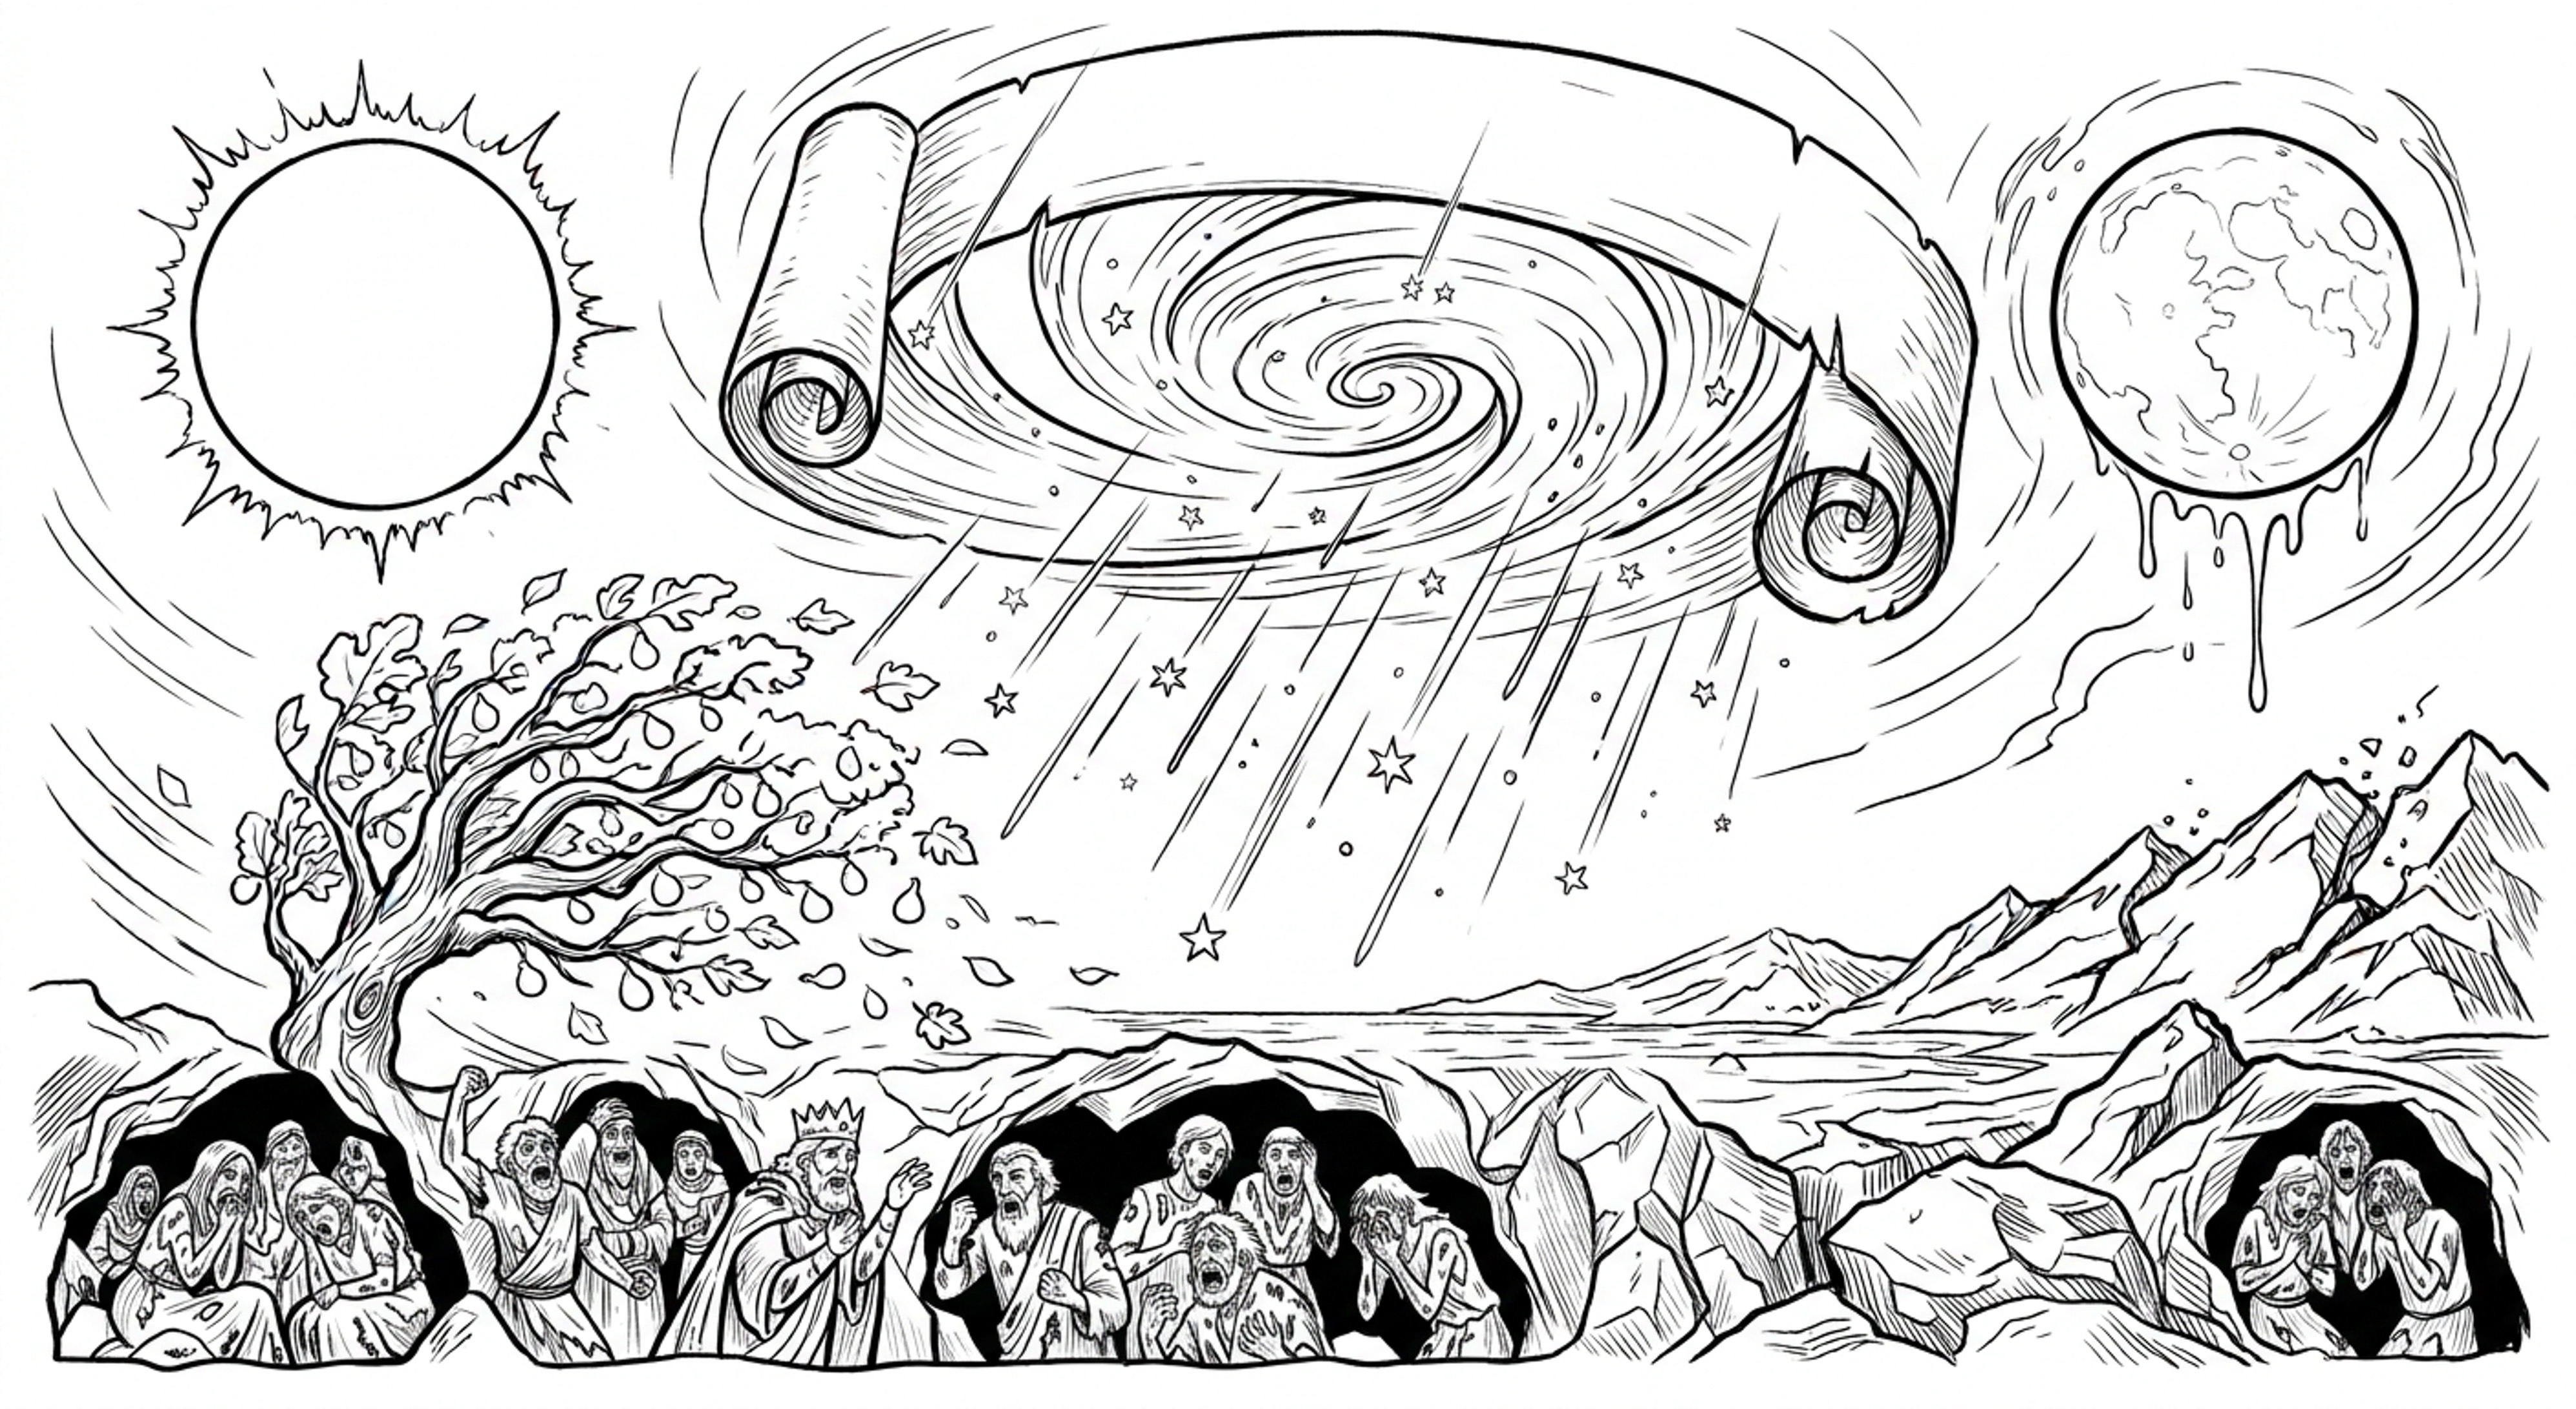
\includegraphics[
    width=1\textwidth, 
    trim=0 0 0 0, 
    clip]{images/seal_6th.jpg}
    \caption{第六印：星辰落地}
    \label{fig:seal_6th}
\end{figure}

我們看到天地震動，地上的人無處可藏，
地上的人恐懼地問，在羔羊公義的憤怒下，誰能站得住？可是到啟示錄第七章我們會看見，那些蒙救贖的人，因為羔羊的血救贖，而得以站立。

{
\small
\renewcommand{\arraystretch}{1}
\begin{center}
\begin{tabular}{ll}
\hline
啟示錄 6:15--17 & 啟示錄 7:9--14 \\
\hline
人躲避上帝和羔羊的面 & 群眾站在上帝和羔羊面前 \\
因忿怒的大日而恐懼 & 穿白衣敬拜上帝 \\
問「誰能站得住？」 & 羔羊的血使蒙救贖人得以站立
\end{tabular}
\end{center}
}

以上的表，可以說是本章主要的信息。
當我們面對羔羊公義的憤怒時，能否坦然站立？
答案不在於我們自己的善行或力量，而在於羔羊已經為我們流血，使我們得蒙救贖、罪得潔淨。

今天，基督仍向我們發出恩典的邀請。
願此書的讀者都接受羔羊的邀請，
不要等到那日才恐懼躲避。
如果你願意的話，現在就悔改、信靠祂的救恩。
因羔羊的恩典，你我都成為那群穿著白衣、站在祂面前，將榮耀和頌讚歸給上帝的人。

\begin{ReaderQuestion}
第六印為什麼使地上的人恐懼？「誰能站得住呢？」這個問題對今天的我們有什麼提醒？
\end{ReaderQuestion}

\subsection*{第一到第六印與馬太福音24章對應}

耶穌在馬太福音24章講的「橄欖山預言」（Olivet Discourse），與啟示錄的第一到第六印，有非常明顯的對應，我列表\ref{tab:seals-matthew24-zh}。

{
\small
\renewcommand{\arraystretch}{1}
\begin{longtable}{p{0.3\textwidth}p{0.4\textwidth}p{0.2\textwidth}}
\caption{啟示錄6章的六印與馬太福音24章的預兆}
\label{tab:seals-matthew24-zh} \\
\hline
\ding{172}-\ding{177}印 & 馬太福音 24 章 & 對應 \\
\hline
\ding{172}白馬，騎馬者出去勝了又要勝 & \textsuperscript{4-5}有人冒基督的名來，迷惑多人 & 假基督、假和平。 \\
\hline
\ding{173}紅馬，奪去太平，使人彼此相殺 & \textsuperscript{6-7}打仗和打仗的風聲，民要攻打民，國要攻打國 & 戰爭、暴力與社會動盪。 \\
\hline
\ding{174}黑馬，天平、糧食昂貴 & \textsuperscript{7}多處必有饑荒 & 糧食短缺及經濟壓力。 \\
\hline
\ding{175}灰馬，死亡及陰間的權柄 & \textsuperscript{7-9}饑荒、地震，並有信徒被交在患難中 & 死亡、災難及苦難。 \\
\hline
\ding{176}殉道者呼求伸冤 & \textsuperscript{9-13}信徒遭患難、被殺、被恨惡，並要忍耐到底 & 信徒受逼迫、殉道及忍耐。 \\
\hline
\ding{177}地震、日月變色、星辰墜落 & \textsuperscript{29-30}日月昏暗、星辰墜落，人子顯在天上 & 同左 \\
\hline
\end{longtable}
}

馬太福音二十四章與啟示錄七印的異象，各有自己的重點。馬太福音強調門徒要謹慎、忍耐到底，並等候人子的來臨。啟示錄進一步以羔羊揭開書卷的異象，表明歷史與審判都在基督的主權之下。

\section{第七印}

\begin{ScriptureBox2}
\item[8:1] 羔羊揭開第七印的時候、天上寂靜約有二刻。
\end{ScriptureBox2}

第七印是在啟示錄8:1，我們放在這裡，與前面六印一起介紹。

第七印沒有像前六印一樣，直接呈現一項災難，而是引出七號的異象（8:2）。七號接續展開上帝的審判，將異象帶入新的階段。

羔羊揭開第七印時，天上寂靜約有二刻。這寂靜如同交響樂中的休止符。眾天使屏息安靜，整個天庭彷彿都在等候，預備迎接接下來大而可畏的審判樂章。這不是審判的終止，而是更猛烈的審判即將展開之前，莊嚴而令人敬畏的停頓。

\subsection*{七印、七號、七碗的順序}

第七印引出七號，第七號吹響時，天上宣告上帝和基督的國度，並提到上帝的忿怒、審判死人及賞賜眾先知和聖徒（11:18）。

但第七號之後沒有立即進入七碗。中間有第12至14章的異象，包括婦人與龍、兩個獸、羔羊與十四萬四千人，以及三位天使的信息。到第15章，約翰看見七位天使拿著末了的七災，並說：「因為　神的大怒在這七災中發盡了。」（15:1）第16章才正式描述七碗倒下。

為了給讀者預覽，我用圖\ref{fig:seals_trumpets_bowls} 解釋七印、七號、七碗的順序。也在下一段順便解釋有關的問題。
\begin{figure}[htbp]
    \centering
    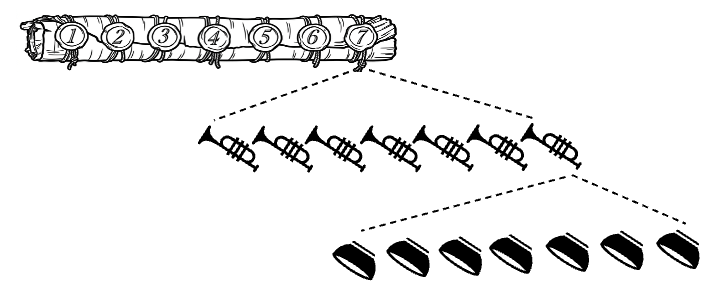
\includegraphics[
    width=1\textwidth, 
    trim=0 0 0 0, 
    clip]{images/seals_trumpets_bowls.png}
    \caption{七印、七號、七碗的順序}
    \label{fig:seals_trumpets_bowls}
\end{figure}

因為七印、七號、七碗有許多審判似乎是類似的場景，就自然的產生了以下的問題。

\begin{InDepth}
\InDepthHeading{七印、七號、七碗是連續發生，還是重述同一個末日審判？}

從字面上來讀，七印、七號、七碗是前後依續發生的。但是會不會是同樣的事件，只是重述，並逐步加深呢？因此，解經者對這三組異象的時間關係，主要有以下兩種理解。

% The table is built row by row, so the box can break between rows.
\par\medskip
{\small\renewcommand{\arraystretch}{1}\setlength{\tabcolsep}{4pt}%
\noindent\begin{minipage}{\linewidth}
\centering
\captionof{table}{七印、七號、七碗的兩種解讀}
\label{tab:seals-trumpets-bowls-zh}
\noindent\rule{\linewidth}{0.4pt}%
\InDepthRow{}{不同審判依序發生}{同樣的審判重述加深}
\InDepthRow{七印}{引出七號。}{敘述上帝的審判。}
\end{minipage}
\InDepthRow{七號}{承接第七印。}{另一角度重述加深審判。}
\InDepthRow{七碗}{承接七號，神的忿怒完全展現。}{再次重述審判。}
\InDepthRow{依據}{第七印引出七號；七號之後出現七碗。}{第六印、第七號、第七碗都出現終局性審判語言。}
\InDepthRow{優點}{重視經文清楚的先後次序。}{能解釋反覆出現的天地震動、上帝忿怒及列國受審判。}
}
\par\medskip

這兩種理解並非在所有方面完全互斥。而採取重述觀點的解經者，也不一定否認經文所呈現的次序。
因此，我們不宜只根據異象的排列，便將每一災精確對應到某個現代歷史事件。
\end{InDepth}

還有，這七印將會如何發生呢？
是在末世大災難期間才會到來，
或是從使徒時代已經開始，一直延伸至基督再來。
或是歷史上反覆出現？
這在神學家有幾個解釋。我特別放在「附錄：各種末世論觀點」。


現在我們繼續讀啟示錄第七章。啟示錄第七章講到有十四萬四千受印，然後有數不清的、各國各族各民各方來的，站在寶座和羔羊面前。

\section{永生神的印保守神的僕人}

\begin{ScriptureBox2}{四位天使執掌著什麼？在地、海和樹木受傷害以前，必須先發生什麼事？}
\item[7:1] 此後我看見四位天使站在地的四角、執掌地上四方的風、叫風不吹在地上、海上、和樹上。

\item[7:2] 我又看見另有一位天使、從日出之地上來、拿著永生　神的印．他就向那得著權柄能傷害地和海的四位天使、大聲喊著說、

\item[7:3] 地與海並樹木、你們不可傷害、等我們印了我們　神眾僕人的額。
\end{ScriptureBox2}

你可能會注意到，在第六印與第七印之間，
怎麼突然插入啟示錄第七章，敘述永生神的印保守神的僕人？

\begin{figure}[htbp]
    \centering
    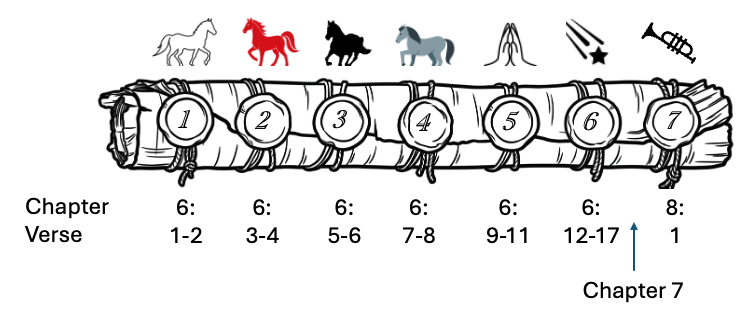
\includegraphics[
    width=1\textwidth,
    trim=0 0 0 0,
    clip]{images/chapter7_insert.png}
    \caption{第六印與第七印之間插入的第七章}
    \label{fig:chapter7_insert}
\end{figure}

這是因為啟示錄6:17以一個尖銳的問題結束：「因為他們忿怒的大日到了，誰能站得住呢？」啟示錄第七章立刻回答這個問題。只有受印的神的僕人以及穿著白衣的數不清的人可以站在寶座和羔羊面前。\footnote{Beale, G. K. (1999).}

「四方的風」是古代舊約常用的語彙，用以表達涵蓋全地的力量。\footnote{但以理書7:2「天的四風颳在大海之上。」耶利米書49:36：「神要使四方的風臨到以攔，將其分散到天下各方。」}因此，此處無須從現代地球幾何或氣象學的角度，質疑「地的四角」與「四方的風」的字面合理性。這裡的重點是神對全地及審判時機的主權。

為什麼先印額，然後施行審判？這是重點。神的印記不是審判的附屬物，而是審判中的身分辨認與救贖安排。我們來看是哪些人受印。

\section{以色列十二支派}

\begin{ScriptureBox2}{數一數支派的數目和每個支派受印的人數。哪一個支派最先被提到？受印的共有多少人？}
\item[7:4] 我聽見以色列人、各支派中受印的數目、有十四萬四千。

\item[7:5] 猶大支派中受印的有一萬二千．流便支派中有一萬二千．迦得支派中有一萬二千．

\item[7:6] 亞設支派中有一萬二千．拿弗他利支派中有一萬二千．瑪拿西支派中有一萬二千．

\item[7:7] 西緬支派中有一萬二千．利未支派中有一萬二千．以薩迦支派中有一萬二千．

\item[7:8] 西布倫支派中有一萬二千．約瑟支派中有一萬二千．便雅憫支派中受印的有一萬二千．
\end{ScriptureBox2}

這裡記載著十四萬四千人受印。他們是誰？這個數字可以是照字面解釋，或也很可能是有象徵的意義。所以一般有三種解釋如表\ref{tab:144000-zh}。

\begin{table}[htbp]
\centering
\renewcommand{\arraystretch}{1}
\caption{十四萬四千人的三種解釋}
\label{tab:144000-zh}
\begin{tabular}{p{2.2cm} p{6.8cm}}
\hline
解釋 & 內容 \\
\hline
以色列 & 指末世從以色列十二支派中受印的十四萬四千人。 \\
象徵教會 & 指由猶太人與外邦信徒組成、屬於神的完整的子民。 \\
象徵以色列 & 以以色列支派象徵末世神的子民，強調神完整地保守祂的子民。 \\
\hline
\end{tabular}
\end{table}





就啟示錄整體而言，十二這個數字反覆出現：十二支派、十二使徒、十二個門、十二個根基，以及新耶路撒冷的十二個城門（啟示錄21:12--14）。
因此，十四萬四千的整齊結構，與啟示錄以十二象徵神子民的完整性，有明顯的呼應。
有些文章試圖直接對應哪一些人才是這十四萬四千人，這裡似乎也不太適合做此對應。
這段經文所強調的重點是神認識屬於祂的子民，並且在審判臨到之際，仍然記念、保守他們。

\section{萬國萬民的敬拜與羔羊的救恩}

\begin{ScriptureBox2}{圈出描述這群人從哪裡來的四個詞，並劃出他們所穿的和手裡所拿的。他們說救恩歸與誰？}
\item[7:9] 此後、我觀看、見有許多的人、沒有人能數過來、是從各國各族各民各方來的、站在寶座和羔羊面前、身穿白衣、手拿棕樹枝．

\item[7:10] 大聲喊著說、願救恩歸與坐在寶座上我們的　神、也歸與羔羊。

\item[7:11] 眾天使都站在寶座和眾長老並四活物的周圍、在寶座前、面伏於地、敬拜　神、

\item[7:12] 說、阿們．頌讚、榮耀、智慧、感謝、尊貴、權柄、大力、都歸與我們的　神、直到永永遠遠。阿們。
\end{ScriptureBox2}

這是多麼壯觀的畫面，那是興奮、有秩序、唱歌的人流。各國各族各民各方的被救贖的人，真正的合一。

\begin{ReaderQuestion}
你得救了嗎？你是不是有確信，將來的你，就會在那個壯闊的人流裡？
如果你還沒有接受基督的救恩，今天就是一個可以認真思想、轉向祂的時刻。耶穌基督為罪人捨命，又從死裡復活；祂邀請你悔改、信靠祂，領受祂白白賜下的恩典。
現在我邀請你接受祂的恩典好嗎？
\end{ReaderQuestion}

我特別寫了以下有關的問題，放在「附錄：常見的問題」：
\begin{itemize}
\item 當你深愛的弟兄（或是姐妹）離世了，可是你走不出傷痛，如何面對？
\item 當復活的時候，人也不娶也不嫁，乃像天上的使者一樣（馬太福音 22:30）
\item 如果將來我在天國，所愛的家人卻不在那裡，我還能快樂嗎？
\end{itemize}

\section{從大患難到永恆安息}

\begin{ScriptureBox2}{劃出這些穿白衣的人是從哪裡來的，以及他們的衣裳是怎樣洗白淨的。然後圈出神和羔羊要為他們所做的一切。}
\item[7:13] 長老中有一位問我說、這些穿白衣的是誰、是從那裡來的。

\item[7:14] 我對他說、我主、你知道．他向我說、這些人是從大患難中出來的、曾用羔羊的血、把衣裳洗白淨了。

\item[7:15] 所以他們在　神寶座前、晝夜在他殿中事奉他．坐寶座的要用帳幕覆庇他們。

\item[7:16] 他們不再飢、不再渴．日頭和炎熱、也必不傷害他們．

\item[7:17] 因為寶座中的羔羊必牧養他們、領他們到生命水的泉源．　神也必擦去他們一切的眼淚。
\end{ScriptureBox2}

血通常使衣裳染紅，可是這裡說，羔羊的血使衣裳洗白淨。在以賽亞書1:18也說到：「你們的罪雖像硃紅、必變成雪白．雖紅如丹顏、必白如羊毛。」

這裡所描繪的得勝，不是信徒憑自己的力量逃離患難，而是羔羊藉著祂的血成就救贖，使神的子民得以進入祂永恆的同在。

\begin{ReaderQuestion}
羔羊的血使衣裳洗白淨，這如何幫助我們理解基督的救恩，並應用在日常生活中？
\end{ReaderQuestion}

從出埃及的拯救，到先知的復興應許，再到羔羊的犧牲與新創造，整個救贖歷史都指向同一個終極盼望：神親自作祂子民的神，羔羊親自作他們的牧者，並擦去他們一切的眼淚。\footnote{
吳榮滁，〈《啟示錄》第12集：額頭蓋印免受傷害〉，台北懷恩堂，2021年9月1日，
https://www.gbc.org.tw/2021/09/20210902/。}
